
\begin{center}
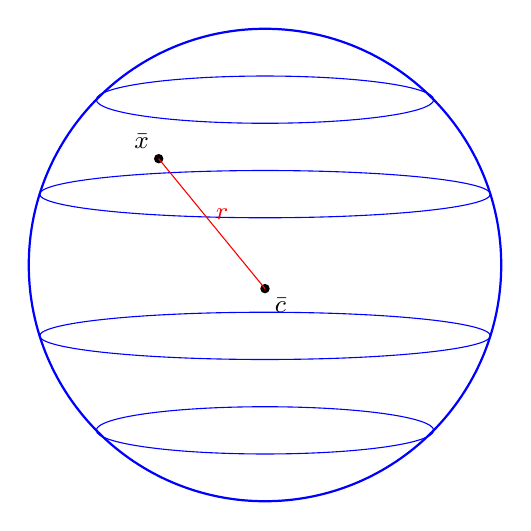
\begin{tikzpicture}[scale=3]
    

  % Outer Sphere
  \shade[ball color=white, opacity=0.0] (0,0) circle(1); % invisible shading
  \draw[blue, thick] (0,0) circle(1); % sphere boundary

  % Latitude lines (ellipses)
  \foreach \y in {-0.7,-0.3,0.3,0.7}
    \draw[blue, thin] (0,\y) ellipse ({sqrt(1 - \y*\y)} and 0.1);

  % Points
  \coordinate (C) at (0,-0.1);
  \coordinate (X) at (-0.45,0.45);
  \fill (C) circle (0.02) node[below right] {\small$\bar{c}$};
  \fill (X) circle (0.02) node[above left] {\small$\bar{x}$};

  % Radius
  \draw[red, thin] (C) -- (X) node[midway, above right=-2pt] {\small$r$};


\end{tikzpicture}

\end{center}